\documentclass[11pt]{article}

\usepackage{fontspec,xunicode}
\setmainfont{Tahoma}
\usepackage[slantfont,boldfont]{xeCJK}
\usepackage{xcolor}                 % replace by the encoding you are using
\setCJKmainfont{Adobe Song Std L}
\usepackage{CJK}
\usepackage{amsmath}
\usepackage{amssymb}
\usepackage{amsfonts}
\usepackage{tocloft}
\usepackage{float}
\usepackage{graphicx}
\usepackage[bookmarks=true]{hyperref}
\usepackage{fancyhdr}

\pagestyle{fancy}
\fancyhead[L]{Machine Learning}
\fancyhead[C]{Note}
\fancyhead[R]{Lanxiao Bai}
\title{Machine Learning Note}
\author{Lanxiao Hermite Bai}
\date{\today}


\begin{document}
\maketitle
\newpage
\tableofcontents
\newpage

\section{基于判别式的分类}
\subsection{线性判别式(Linear discriminant)}
	定义线性判别式为:
	\begin{align}
		&g_i(\mathbf{x} | \mathbf{w}_i, w_0) = \mathbf{w}_i^T\mathbf{x} + w_0\nonumber\\
		&\phantom{g_i(\mathbf{x} | \mathbf{w}_i, w_0)} = \sum_{j = 1}^d w_{ij}x_j + w_{i0}\nonumber
	\end{align}
	\begin{itemize}
		\item 优点: 复杂度低-$O(d)$
		\item 缺点: 因为线性,不够灵活
	\end{itemize}
	
	解决方法:
	\begin{enumerate}
		\item 二次判别式: \[g_i(\mathbf{x} | \mathbf{W}_i, \mathbf{w}_i, w_{i0}) = \mathbf{x}\mathbf{W}^T_i\mathbf{x} + \mathbf{w}_i\mathbf{x} + w_{i0}\]
		\item 高阶项(high-order term)和非线性基函数(non-linear basis function)的线性组合
	\end{enumerate}
	
	\[g_i(x) = \sum_{j = 1}^k w_j\phi_{ij}(x)\]
	
	缺点:
	\begin{itemize}
		\item 计算复杂度较高-$O(d^2)$
		\item 偏倚方差两难选择-小样本下容易过拟合(overfitting)
	\end{itemize}
	\subsection{梯度下降法(Gradient Descent)}
	\subsubsection{2类问题}
		定义Logistic函数:
			\[\mathrm{sigmoid}(y) = \frac{1}{1 + e^{-y}}\]
		Logistic函数将判别式的数值变换为后验概率,则当$P(C_1 | \mathbf{x}) = y = \mathrm{sigmoid}(\mathbf{w}^T\mathbf{x} + w_0) > 0.5$时,取为类别$C_1$.
		
		定义$E(\mathbf{w} | \mathbf{\chi})$表示参数$\mathbf{w}$在给定训练集上的误差等价于
		\[\mathbf{w}^* = \arg\min_w E(\mathbf{w} | \mathbf{\chi})\]
		对于可微函数$E(\mathbf{w} | \mathbf{\chi})$,我们有偏导数组成的梯度向量
		\[\nabla_{\mathbf{w}}E = [\frac{\partial E}{\partial w_1}, \frac{\partial E}{\partial w_2}, \cdots, \frac{\partial E}{\partial w_d}]^T\]
		则更新向量
		\[\Delta \mathbf{w} = -\eta \nabla_{\mathbf{w}}E\]
		\[\mathbf{w} = \mathbf{w} + \Delta \mathbf{w}\]
		
		其中$\eta$称为学习率(learn rate),该参数过大则导致摆动或发散,过小则有可能陷入局部最小值以及收敛太慢.
		
		给定两个类的样本$\chi = \{\mathbf{x}^t, r^t\}$服从伯努利分布,则样本的似然
		\[I(\mathbf{w}, w_0 | \mathbf{\chi}) = \prod_t (y^t)^{(r^t)}(1 - y^t)^{(1 - r^t)}\]
		取对数,则我们可以得到交叉熵(cross-entropy):
		\[E(\mathbf{w}, w_0 | \mathbf{\chi}) = -\sum_t r^t\log y^t + (1 - r^t)\log(1 - y^t)\]
		作为误差函数,得到
		\[\Delta \mathbf{w}_j = -\eta\frac{\partial E}{\partial w_i} = \eta \sum_t (r^t - y^t)x^t_j \]
		为了保证sigmoid函数可以产生足够的梯度,一般从$[-0.01, 0.01]$中随机均匀抽取.
		
	\subsubsection{K类问题}
		定义Softmax函数:
			\[p(C_i | \mathbf{x}) = \frac{e^{y_i}}{\sum_{j = 1}^K e^{y_j}}\]
		
		
		
		给定两个类的样本$\chi = \{\mathbf{x}^t, r^t\}$服从多项分布,则样本的似然
		\[I(\mathbf{w}, w_0 | \mathbf{\chi}) = \prod_t \prod_i(y_i^t)^{(r_i^t)}\]
		取对数,则我们可以得到交叉熵(cross-entropy):
		\[E(\mathbf{w}, w_0 | \mathbf{\chi}) = -\sum_t \sum_i \log y_i^t\]
		\[\frac{\partial y_i}{\partial a_j} = y_i(\delta_{ij} - y_i)\]
		作为误差函数,得到
		\[\Delta \mathbf{w}_j = -\eta\frac{\partial E}{\partial w_i} = \eta \sum_t (r^t - y^t)x^t_j \]
\section{决策树(Decision Tree)}
	\begin{itemize}
		\item 优点: \begin{enumerate}
						\item 决策层次能够快速安排,$O(\log n)$
						\item 可解释性好,可以转换成一组IF-THEN规则 
						\item 即可以处理数值型数据也可以处理类别型数据
					\end{enumerate}
		\item 缺点: \begin{enumerate}
						\item 训练一棵最优的决策树是一个完全NP问题(实际应用时决策树的训练采用启发式搜索算法例如 贪心算法 来达到局部最优。)
						\item 决策树创建的过度复杂会导致无法很好的预测训练集之外的数据, 从而导致过拟合(overfitting)
						\item 有些问题决策树没办法很好的解决,例如 异或问题
					\end{enumerate}
	\end{itemize}
	\subsection{分类树}
		在用于分类的决策树中,划分的优劣用不纯性度量(impurity measure):
		\begin{enumerate}
			\item 熵函数(entropy): \[L_m = -\sum_{i = 1}^K p_m^i \log_2 p_m^i\]
			\item 基尼系数(Gini index): \[\phi(p_1, p_2, \cdots, p_K) = 1 - \sum_{i = 1}^K p^2_i\]
			\item 误分类误差: \[\phi(p_1, p_2, \cdots, p_K) = 1 - \max(p_i)\]
			\item 其他, 满足规则: \begin{enumerate}
									\item 对于任意$p \in [0, 1]$, \[\phi(1/K, 1/K, \cdots, 1/K) = \phi(p_1, p_2, \cdots, p_K)\]
									\item \[\phi(1, 0, \cdots, 0) = \phi(0, 1, \cdots, 0) = \phi(0, 0, \cdots, 1) = 0\]
									\item 在$p \in [0, 1/2]$上递增, 在$p \in [1/2, 1]$上递减
		 						\end{enumerate}
		 \end{enumerate}
		 
		 对于以上不纯性度量计算出的结果,决策树算法递归地选择使得信息增益最大的属性进行节点的分裂:
		 \begin{enumerate}
		 	\item CART:使用信息增益作为分裂的规则,信息增益越大,则选取该分裂规则
		 	\item C4.5:选择了信息增益率替代信息增益
		 	\item ID3:以基尼系数替代熵,最小化不纯度而不是最大化信息增益。
		 \end{enumerate}
	\subsection{回归树}
		回归树以和分类树相同的方式构造, 不纯性量度改为适合回归的度量方法,定义
		\[b_m(\textbf{x}) = \left\{\begin{array}{ll}
									1 & \textrm{if\ } \textbf{x} \in \chi_m: \textbf{x} \textrm{\ reaches\ node\ }m\\
									0 & \textrm{otherwise}
								  \end{array}\right.\]
								  
		用均方误差估计划分的好坏:\[E_m = \frac{1}{N_m} \sum_t (r^t - g_m)^2b_m(\textbf{x}^t)\]
		
		\[g_m = \frac{\sum_t b_m(\textbf{x}^t)r^t}{\sum_tb_m(\textbf{x}^t)}\]					
	\subsection{剪枝}
		为了克服决策树的过拟合问题,我们使用剪枝(pruning)控制树的大小:
		\begin{itemize}
			\item 先剪枝(prepruning):在树完全构造出来之前停止树的构造
			\item 后剪枝(postpruning):在树完全生长之后剪枝,去掉不必要的子树
		\end{itemize}
		
	\subsection{随机森林(Random Forest)}
		为了克服决策树的过拟合问题,我们也可以随机划分数据集,构建多棵决策树,最后投票表决结果.
		优点:\begin{itemize}
				\item 对于很多种资料,它可以产生高准确度的分类器
				\item 它可以处理大量的输入变数
				\item 它可以在决定类别时,评估变数的重要性
				\item 在建造森林时,它可以在内部对于一般化后的误差产生不偏差的估计
				\item 对于不平衡的分类资料集来说,它可以平衡误差
				\item 它计算各例中的亲近度,对于数据挖掘、侦测偏离者(outlier)和将资料视觉化非常有用
				\item 学习过程很快速 
			\end{itemize}
			
	\section{感知机和人工神经网络(Artificial Neural Network)}
	\subsection{感知器(Perceptron)}
		感知器是人工神经网络的基本处理元素,它具有输入,其输入可能来自于环境或者其他感知器的输入。与每个输入$x_i \in \mathbb{R}(j = 1, 2, \cdots, d)$相关联的是一个连接权重(connection weight)或触突权重(synaptic weight)$w_j = \mathbb{R}$, 而输出$y$在最基本的情况下即为输入的加权和。
			\[y = \sum_{j = 1}^d w_jx_j + w_0 = \mathbf{w}^T\mathbf{x}\]
			其中$\mathbf{w} = [w_0, w_1, \cdots, w_d]^T, \mathbf{x} = [1, x_1, \cdots, x_d]^T$。
			
			我们用激活函数确认类的划分:
			\begin{enumerate}
				\item Sigmoid函数:\[z = \frac{1}{1 + e^{-y}}\] \begin{itemize}
								\item 优点:能够把输入的连续实值“压缩”到0和1之间
								\item 缺点: \begin{itemize}
												\item Sigmoids saturate and kill gradients.
												\item Sigmoid 的 output 不是0均值
											\end{itemize}
										\end{itemize}
				\item Tanh函数:\[\tanh(x) = 2\mathrm{sigmoid}(2x)-1\]
				\item ReLU函数:\[ReLU(x) = \max(0, x)\] \begin{itemize}
					\item 优点: \begin{itemize}
									\item Krizhevsky et al. 发现使用 ReLU 得到的SGD的收敛速度会比 sigmoid/tanh 快很多(看右图)。有人说这是因为它是linear,而且 non-saturating
									\item 相比于 sigmoid/tanh,ReLU 只需要一个阈值就可以得到激活值,而不用去算一大堆复杂的运算
								\end{itemize}
					\item 缺点: 训练的时候很"脆弱",如果一个非常大的梯度流过一个 ReLU 神经元,更新过参数之后,这个神经元再也不会对任何数据有激活现象了。
							\end{itemize}
			\end{enumerate}
			\begin{figure}[H]
        		\begin{center}
        			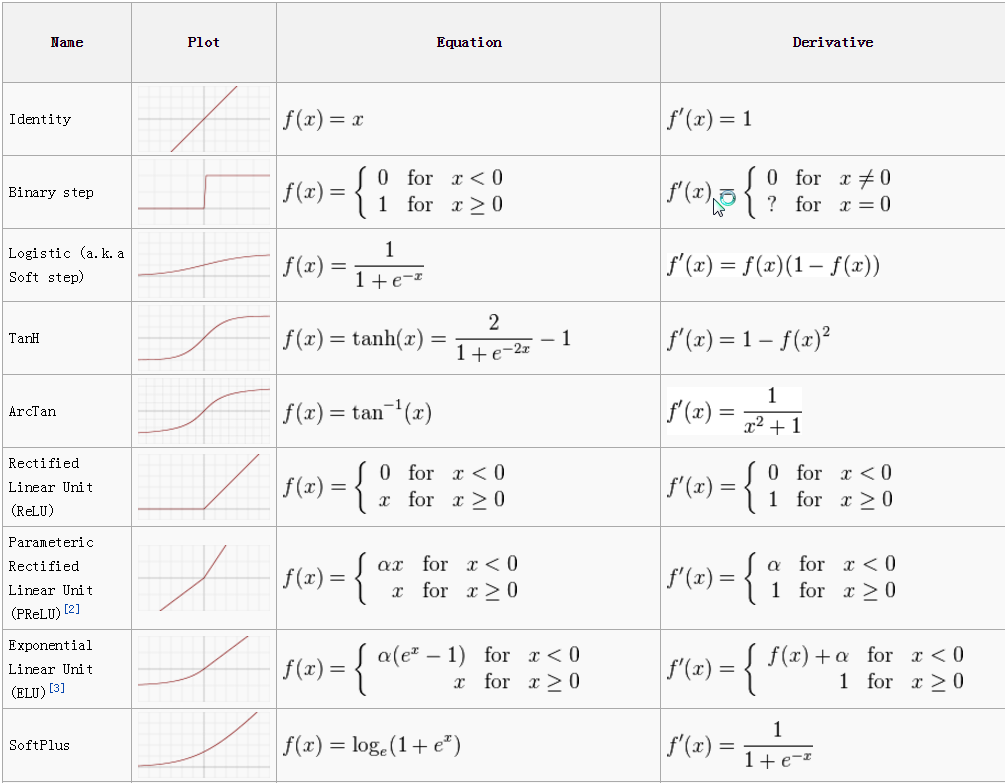
\includegraphics[width=8cm]{./imgs/ac1.png}
        			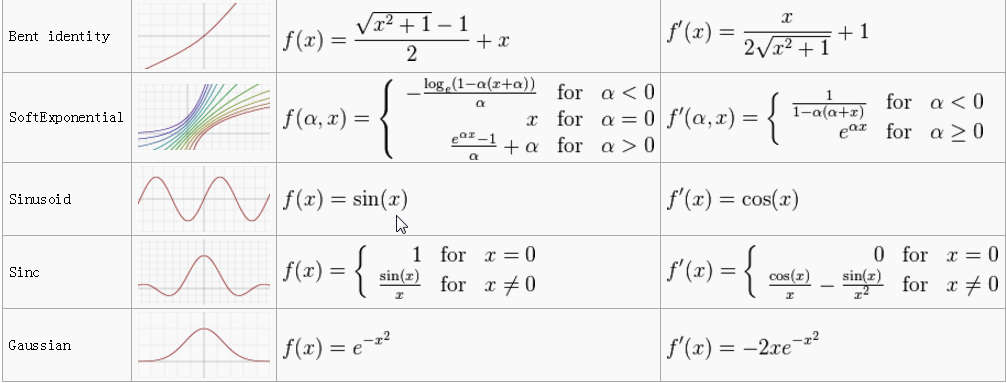
\includegraphics[width=8cm]{./imgs/ac2.png}
        			\caption{常见的激活函数}
        		\end{center}
    		\end{figure}
    		
    		当存在$K > 2$个输出时,有$K$个感知器,每个都具有权重向量$\mathbf{w}_i$
    		\[y_i = \sum_{j = 1}^d w_{ij}x_j + w_{i0} = \mathbf{w}^T_i\mathbf{x}\]
    		\[\mathbf{y} = \mathbf{Wx}\]
    		
    		\subsection{多层感知器}
    			多层感知器(MLP)是在单层感知器中插入了一层或多层中间层或隐藏层(hidden layer)以用于实现非线性的判别式或回归。
    			
    			以只有一个隐藏层的神经网络为例,
    			\[z_h = \mathrm{sigmoid(\mathbf{w}_h^T\mathbf{x})}, h = 1, \cdots, H\]
    			\[y_i = \mathbf{v}_i^T\mathbf{z} = \sum_{h = 1}^H v_{ih}z_{h} + v_{i0}\]
    		\subsection{后向传播算法(BP)}
    			我们用微分链式法则(Chain Rule)计算对应参数$w_{hj}$
    			\[\frac{\partial E}{\partial w_{hj}} = \frac{\partial E}{\partial y_i} \frac{\partial y_i}{\partial z_h} \frac{\partial z_h}{\partial w_{hj}}\]的梯度,从而使用梯度下降进行优化。
    			\subsubsection{非线性回归}
    				使用平方误差函数作为样本上的误差衡量
    				\[E(\mathbf{W, v | \chi}) = \frac{1}{2}\sum_t (r^t - y^t)^2\]
    				则第二层的权重变化为
    				\[\Delta v_h = \eta \sum_t (r^t - y^t)z_h^t\]
    				而输入层则为
    				\begin{align}
    					&\Delta w_{hj} = -\eta \frac{\partial E}{\partial w_{hj}}\nonumber\\
    					&\phantom{\Delta w_{hj}} = -\eta \sum_t  \frac{\partial E^t}{\partial y^t} \frac{\partial y^t}{\partial z_h^t} \frac{\partial z_h^t}{\partial w_{hj}}\nonumber\\
    					&\phantom{\Delta w_{hj}} = \eta \sum_t (r^t - y^t)v_hz_h^t(1 - z_h^t)x_j^t\nonumber
    				\end{align}
    				
    				当我们同时学习多个回归问题,我们有
    				\[y_i^t = \sum_{h = 1}^H v_{ih}z_{h}^t + v_{i0}\]
    				\[E(\mathbf{W, V | \chi}) = \frac{1}{2} \sum_t \sum_i (r_i^t - y_i^t)^2\]
    				所以
    				\[\Delta v_h = \eta \sum_t (r^t - y^t)z_h^t\]
    				\[\Delta w_{hj} = \eta \sum_t \left[\sum_i (r^t - y^t)v_{ih}\right]z_h^t(1 - z_h^t)x_j^t\]
    			\subsubsection{2类判别式}
    				对于输出单元
    				\[y^t = \mathrm{sigmoid}(\sum_{h = 1}^H v_{ih}z_{h} + v_{i0})\]
    				有
    				\[E(\mathbf{W, V | \chi}) = - \sum_t r^t \log y^t + (1 - r^t)\log (1 - y^t)\]
    				根据梯度下降,得到
    				\[\Delta v_h = \eta \sum_t (r^t - y^t)z_h^t\]
    				\[\Delta w_{hj} = \eta \sum_t (r^t - y^t)v_hz_h^t(1 - z_h^t)x_j^t\]
    			\subsubsection{多类判别式}
    				\[o_i^t = \sum_{h = 1}^H v_{ih}z_{h}^t + v_{i0}\]
    				\[y^t_i = \frac{\exp o_i^t}{\sum_k \exp o_k^t}\]
    				则误差函数是
    				\[E(\mathbf{W, V | \chi}) = - \sum_t \sum_i r^t_i \log y^t_i\]
    				所以
    				\[\Delta v_h = \eta \sum_t (r^t - y^t)z_h^t\]
    				\[\Delta w_{hj} = \eta \sum_t \left[\sum_i (r^t - y^t)v_{ih}\right]z_h^t(1 - z_h^t)x_j^t\]
    			\subsubsection{多个隐藏层}
    				如果有多个隐藏层,他们都各自具有自己的权重,如
    				\[z_{1h} = \mathrm{Activate}(\mathbf{w}_{1h}^T\mathbf{x})\]
    				\[z_{2h} = \mathrm{Activate}(\mathbf{w}_{2h}^T\mathbf{z_1})\]
    				\[\vdots\]
    				\[y = \mathbf{v}^T\mathbf{z}_n\]
    				
    				同理,我们可以用BP算法依次计算传播到各层的梯度。
    		\subsection{训练过程}
    			\subsubsection{加速收敛}
    				梯度下降是一个收敛较慢的算法,我们有一些方法可以加速它的收敛。
    				\paragraph{动量(Momentum)}
    					我们将上一次的更新向量加入考虑,用于抵消在错误方向的下降
    					\[\Delta w_i^t = - \eta \frac{\partial E^t}{\partial w_i} + \alpha\Delta w_i^{t - 1}\]
    				\paragraph{Nesterov 动量}
    					在向量向下优化的过程中,我们希望知道能够提前知道在哪些地方会上升,在此之前就开始减速
    				\paragraph{自适应学习率}
    					\[\Delta \eta = \left\{\begin{array}{ll}
    						+ \alpha & \mathrm{if\ }E^{t + \tau} < E^t\\
    						-b \eta & \mathrm{otherwise}
    					\end{array} \right.\]
    			\subsubsection{防止过拟合}
    				防止过拟合有以下几种方法:
    				\begin{enumerate}
    					\item 在适度的时间停止训练
    					\item Dropout: 是指在模型训练时随机让网络某些隐含层节点的权重不工作
    					\item 选择适当的隐层数量
    					\item 正则化(Regularization):在误差函数上加上惩罚项
    				\[\tilde{E}(\mathbf{w, X, y}) = E(\mathbf{w, X, y}) + \alpha \Omega(\mathbf{w})\]
    				\begin{itemize}
    					\item $L^2$正则化:\[\Omega(\mathbf{w}) = \frac{\mathbf{w}^T\mathbf{w}}{2}\]
    					\item $L^1$正则化:\[\Omega(\mathbf{w}) = ||\mathbf{w}||_1 = \sum_i |\mathbf{w}_i|\]
    				\end{itemize}
    				\end{enumerate}
		\subsubsection{应用与扩展}
			\paragraph{卷积神经网络(Convolutional Neural Network)}
			
			在卷积神经网络中,用到了以下的几个概念:
			\begin{itemize}
				\item 卷积: 
				在连续的情形下,我们有
				\[s(t) = (x*w)(t) = \int^{\infty}_{-\infty} x(a)w(t-a)da\]
				在离散的情形下,我们有
				\[s(t) = (x*w)(t) = \sum_{-\infty}^{\infty} x(a)w(t-a)\]
				在神经网络中,我们用互相关函数完成卷积的操作
				\[S(i, j) = (I*K)(i, j) = \sum_m \sum_n I(i + m, j + n)K(m, n)\]
				\begin{figure}[H]
        			\begin{center}
        				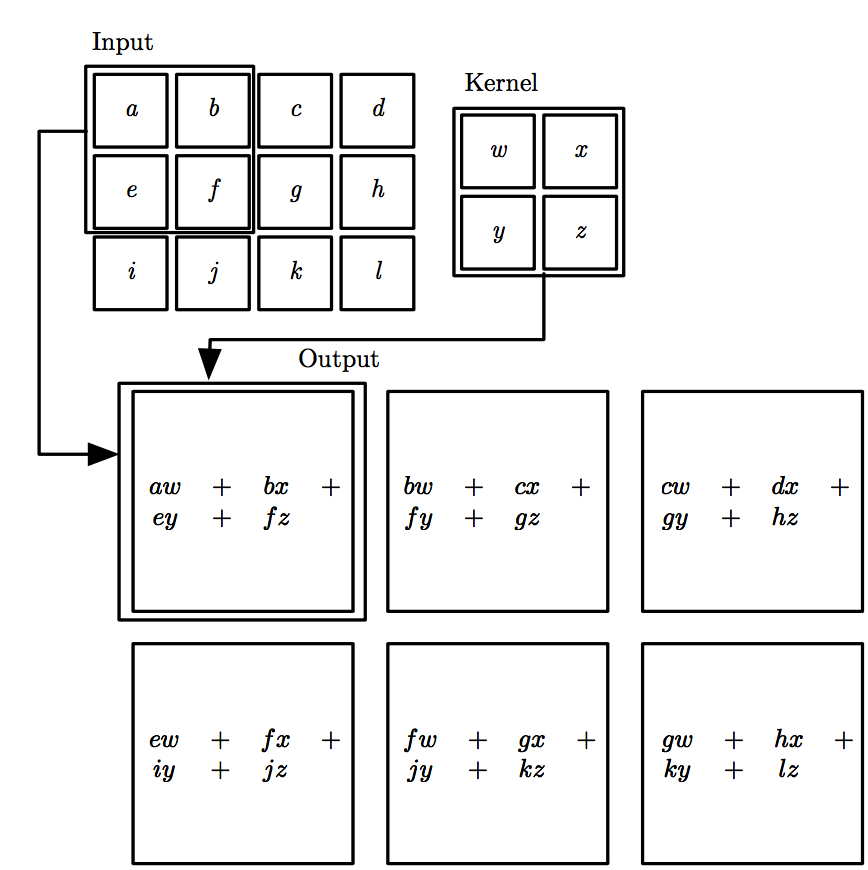
\includegraphics[width=8cm]{./imgs/conv.png}
        				\caption{卷积操作}
        			\end{center}
    			\end{figure}
    			\item 稀疏交互(Sparse interaction):核的规模远小于输入的规模来实现,从而只需要更少的计算量
    			\item 参数共享(parameter sharing):在一个模型的多个函数中使用相同的参数
    			\item 对平移等变(equivariant):一个函数满足输入改变,输出也以同样的方式改变这一性质
    			\item 池化(Pooling):池化层往往在卷积层后面,通过池化来降低卷积层输出的特征向量,同时改善结果(不易出现过拟合)。使用池化可以看作是增加了一个无限强的先验:卷积层学得的函数必须具有对 少量平移的不变性。当这个假设成立时,池化可以极大地提高网络的统计效率。
    			 
    			最常见的池化操作为平均池化mean pooling和最大池化max pooling:
    			\begin{itemize}
    				\item 平均池化:计算图像区域的平均值作为该区域池化后的值。
					\item 最大池化:选图像区域的最大值作为该区域池化后的值。
				\end{itemize}
    		
			\end{itemize}
\end{document}
